\subsection{EXTENSIONS}

DEFINITION 5. Let \(\mathfrak{a}\) and \(\mathfrak{b}\) be two Lie algebras over \(\mathbf{K}\) . An extension of \(\mathfrak{b}\) by \(\mathfrak{a}\) is a sequence:

\[
a \xrightarrow {\lambda} g \xrightarrow {\mu} b
\]

where g is a Lie algebra over K, μ a surjective homomorphism of g onto b and λ an injective homomorphism of a onto the kernel of μ.

The kernel \(\mathfrak{n}\) of \(\mu\) is called the kernel of the extension. The homomorphism \(\lambda\) is an isomorphism of \(\mathfrak{a}\) onto \(\mathfrak{n}\) and the homomorphism \(\mu\) defines an isomorphism of \(\mathfrak{g} / \mathfrak{n}\) onto \(\mathfrak{b}\) when passing to the quotient.

By an abuse of language, g is also called an extension of b by a.

Two extensions:

\[
a \xrightarrow {\lambda} g \xrightarrow {\mu} b, \quad a \xrightarrow {\lambda^ {\prime}} g ^ {\prime} \xrightarrow {\mu^ {\prime}} b
\]

are said to be equivalent if there exists a homomorphism \(f\) of \(\mathfrak{g}\) into \(\mathfrak{g}'\) such that the following diagram:

\pandocbounded{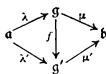
\includegraphics[keepaspectratio]{images/part001_2862d8fe.jpg}}

is commutative (that is such that \(f \circ \lambda = \lambda', \mu' \circ f = \mu\) ). We show that such a homomorphism is necessarily bijective. First \(f\) is injective. For if \(x \in \mathfrak{g}\) is such that \(f(x) = 0\) , then \(\mu(x) = \mu'(f(x)) = 0\) and hence \(x = \lambda(y)\) for some \(y \in \mathfrak{a}\) ; then \(\lambda'(y) = f(\lambda(y)) = f(x) = 0\) , hence \(y = 0\) and hence \(x = 0\) . On the other hand, \(f\) is surjective. For \(\mu' \circ f = \mu\) is surjective and hence \(f(\mathfrak{g}) + \lambda'(\mathfrak{a}) = \mathfrak{g}'\) ; on the other hand \(f(\mathfrak{g}) \supset f(\lambda(\mathfrak{a})) = \lambda'( \mathfrak{a})\) .

It follows from this that the relation just defined between two extensions of b by a is an equivalence relation.

PROPOSITION 6. Let

\[
a \xrightarrow {\lambda} g \xrightarrow {\mu} b
\]

be an extension of b by a and n its kernel.

\begin{enumerate}
\def\labelenumi{(\alph{enumi})}
\item
  If there exists a subalgebra m of g supplementary to n in g, the restriction of μ to m is an isomorphism of m onto b. If v denotes the inverse isomorphism of this restriction, v is a homomorphism of b into g and μ ∘ v is the identity automorphism of b.
\item
  Conversely, if there exists a homomorphism \(v\) of \(\mathfrak{b}\) into \(\mathfrak{g}\) such that \(\mu \circ v\) is the identity automorphism of \(\mathfrak{b}\) , then \(v(\mathfrak{b})\) is a supplementary subalgebra of \(\mathfrak{n}\) in \(\mathfrak{g}\) .
\end{enumerate}

The assertions of (a) are immediate. On the other hand, let v be a homomorphism of b into g such that \(\mu \circ v\) is the identity automorphism of b. Then \(v(b)\) is a subalgebra of g and g is the direct sum of \(v(b)\) and \(\mu^{-1}(0) = n\) (Algebra, Chapter VIII, §1, no. 1).

DEFINITION 6. Let

\[
a \xrightarrow {\lambda} g \xrightarrow {\mu} b
\]

be an extension of \(\mathfrak{b}\) by \(\mathfrak{a}\) and \(\mathfrak{n}\) its kernel. This extension is called inessential (resp. trivial) if there exists a subalgebra (resp. an ideal) of \(\mathfrak{g}\) supplementary to \(\mathfrak{n}\) in \(\mathfrak{g}\) . This extension is called central if \(\mathfrak{n}\) is contained in the centre of \(\mathfrak{g}\) .

If the extension is trivial, let \(m\) be an ideal of \(g\) supplementary to \(n\) in \(g\) . Then (cf.~no. 1) \(g\) is canonically identified with the Lie algebra \(m \times n\) and hence with the Lie algebra \(a \times b\) . Conversely, let \(a\) and \(b\) be two Lie algebras; then \(a \times b\) is a trivial extension of \(b\) by \(a\) .

An inessential central extension is trivial. For let \(\mathfrak{g}\) be a Lie algebra, \(\mathfrak{n}\) an ideal of \(\mathfrak{g}\) contained in the centre of \(\mathfrak{g}\) and \(\mathfrak{m}\) a subalgebra of \(\mathfrak{g}\) supplementary to \(\mathfrak{n}\) in \(\mathfrak{g}\) . Then \([\mathfrak{m},\mathfrak{g}] = [\mathfrak{m},\mathfrak{m}] + [\mathfrak{m},\mathfrak{n}] = [\mathfrak{m},\mathfrak{m}] \subset \mathfrak{m}\) and hence \(\mathfrak{m}\) is an ideal of \(\mathfrak{g}\) .

